\section{Specifications}
\subsection{Size, Weight, Speed}
Below is a list of design specifications for DynaSaRR. Drive wheels with a 12 inch diameter were selected, with inflatable rubber tires for enhanced control while navigating and increased traction during wall traversal. This design choice was intended to reduce slippage and ensure that more torque from the motor would be used to power the wheels than if tires with less traction were used, thereby increasing speed on the ground and obstacle traversing ability. DynaSaRR's chassis was designed to be longer than that of the sample robot in order to accommodate the lifting arm mechanism which would propel it over the wall.

The frame was constructed from T-slotted 80/20 aluminum 6061 extrusions. Two levels of rectangular frame were separated by 3-inch pieces of extrusion, creating two levels onto which parts could be mounted. This shape allowed for maximum organizational efficiency, easy mounting of parts, and modularity, while maintaining a compact, maneuverable chassis.

Based on the initial CAD model, in which a weight estimate was calculated in CREO 5.0 using material assignment and inputting calculated densities of the parts already possessed by the team, including the drill batteries, Teensy board, and various motors, DynaSaRR was specified to weigh 45 lbs. The true weight, measured after the robot was manufactured and assembled, came to 44.3 lbs--very close to the estimated weight. This allowed for precise values to be in the calculations, as the weight of any component or subsystem calculated in CREO could be assumed to be very close to its real weight.


\begin{itemize}
    \item Total Weight: 44.3 lbs
    \item Frame Width: 12 in
    \item Frame Length: 19.5 in
    \item Frame Height: 5 in
    \item Chassis Clearance Height: 3.9 in
    \item Drive Wheel Diameter: 12 in
    \item Drive Wheel Width: 1.7 in
    \item Max SaRR Width: 15 in
    \item Max SaRR Length (Lifting Arms Up): 22 in
    \item Total SaRR Height: 14 in
\end{itemize}

In order to estimate DynaSaRR's speed along a flat surface, it was first necessary to calculate the total force required to maintain speed:
$$F_{tot} = F_r + F_{drag}.$$
$F_r$ is the rolling resistance, and is calculated as $$F_r = c*W,$$ where $c$ is the rolling resistance coefficient of the tires, and $W = m*g$ is the weight of the robot (mass times acceleration due to gravity). $c$ for bike tires on waxed wood was found to be $0.002$, and on asphalt was $0.005$. From these values, $c$ for our tires on linoleum was estimated be $0.004$. The weight of DynaSaRR was 48 lbs. with the med kit, so $F_r$ was calculated as $77.23\frac{lb*in}{s^2}$.
$$ F_{drag} = \frac{C_d*A* \rho_{air}*V^2}{2}.$$
Here, $C_d$ is the coefficient of drag, which was estimated to be 1.16 due to the ratio of length (20in) to height (12in) of approximately 2 of the robot face (calculated for a flat rectangular plate). $A$, the area of the robot, was calculated as $0.3*20*12$, because the SaRRchaeologists estimated that only about $30 \%$ of the 20 by 12 rectangle actually contained material. $\rho_{air} = 4.06*10^-5 \frac{lb}{in^3}$, and $V$ is the velocity of the robot. In order to complete the calculations, the velocity had to be estimated and then the following calculations had to be iterated over until the estimated and calculated velocities matched (detailed calculations are shown in the Appendix). In the final iteration, a velocity of 7mph was assumed, so $F_{drag}$ was calculated as $25.763 \frac{lb*in}{s^2}$. Thus, $F_{tot} = 102.97 \frac{lb*in}{s^2}$. From this, torque was calculated as 
$$ \tau = r_{wheel}*F_{tot}*sin( \theta).$$
Since this calculation was for a flat surface, $\theta = 90 \degree $, and the wheels had a radius of 6 in. Drive train efficiency was estimated to be $84.1 \%$, so actual torque for each of the two driven wheels was calculated as
$$ \tau_{real} = \frac{\tau}{2*0.841} = 367.33 \frac{lb*in^2}{s^2}.$$
This was then multiplied by a safety factor of 2 and converted to Newton-meters, resulting in a torque of $0.22 N*m$. The corresponding RPM (read off Fig. \ref{fig:motorcurve}) at that torque was 4700 rpm, which was converted to a speed by multiplying by the wheel circumference, resulting in a speed estimate of 6.99mph--extremely close to the original estimate. This showed that this iteration of calculations would be an accurate predictor of DynaSaRR's performance: it could be expected to travel at approximately 7mph.

\begin{figure}[ht]
    \centering
    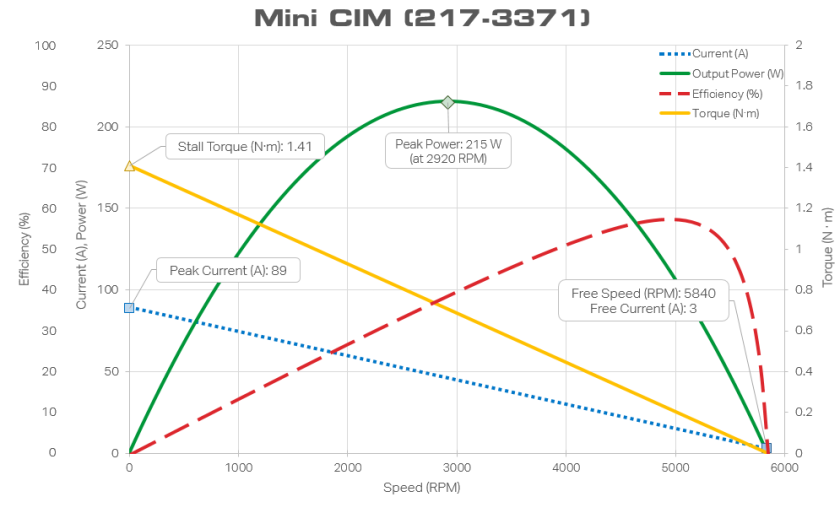
\includegraphics[width=\textwidth]{mini-cim-motor-curve}
    \caption{Motor Curves for the VEX Motors}
    \label{fig:motorcurve}
\end{figure}

DynaSaRR had an estimated top speed of 7.2 mph or 10.56 feet per second. Additionally, the turning radius was calculated to be 19.6 in. As such, moving at top speed, it would take the DynaSaRR approximately 10 seconds to complete the entire course (approximately 100 ft), with the exception of the wall traversal portion. However, this is clearly not a realistic expectation, as the robot would only be moving at top speed for approximately the first 50 feet of the course after picking up the medkit. Based on open- and closed-loop tests, the SaRRchaeologists estimated that it would take DynaSarr approximately 10 seconds to retrieve the medkit, 10 seconds to circumvent the pylon (in addition to the approximately 5 seconds of top-speed driving), 10 seconds to breach the wall, 30 seconds for chute traversal, and 45 seconds for light tracking and medkit placement. Combining these times, the SaRRchaeologists predict that it will take approximately 2 minutes to complete the course

The maximum communication range of the remote control system used was right around 250 ft in ideal testing conditions (a linear, enclosed section of hallway). The SaRR ran through autonomous tasks at any distance from the remote controller. The range of the remote controller batteries was no more than 6 hours of continuous usage. The range till failure of the drill batteries that provided the primary power to the SaRR was about 210 minutes of intermittent task testing (chute navigation, light navigation, wall traversal). However, performance was limited significantly after only 30-45 minutes of intermittent testing. 



\subsection{Operational and Navigational Modes}
The SaRR had two modes of control: open-loop mode, in which it was controlled by inputs to the controller, and autonomous mode, in which it was operated by closed-loop Arduino code sent to a Teensy board. The open-loop navigation was used to locate and retrieve the medkit, then move to the front of the wall obstacle, while the rest of the course was navigated autonomously.

In order to successfully navigate to the medkit, pick it up, and then drive to the front of the wall obstacle, the open-loop remote controller (the human-technology interface in this design) had 4 directional inputs programmed to the right joystick: forward, backward, right turn and left turn. Moving the left joystick vertically triggered the lifting and lowering of the medkit retrieval arm, and horizontal motion controlled the rotation of the lifting arms. The controller also had 2 switches which amplified an isolated channel based on the location of the corresponding knob located on the controller. The right switch triggered autonomous mode. The left switch triggered a reset of several booleans--these could be changed in the code in order to have autonomous mode go directly to a certain function (e.g., skip over the wallTraverse() function and go directly to chuteTraverse()). The signals from the remote controller were obtained on the SaRR by a wireless receiver and were read into the Teensy micro-controller, where actions were assigned based on the values transmitted. In open-loop mode, these were the only inputs received by the SaRR.

When the right shoulder switch was flipped, the value of the designated channel breached a specified input threshold, activating autonomous mode. In autonomous mode, the only inputs to the micro-controller came from three proximity sensors and two light sensors. One proximity sensor was located on the front of the SaRR, and the other two were located on opposite sides of the frame. The two light sensors were located on the top of the bottom beam of the frame and were facing forward. 

When in autonomous mode, the SaRR had to complete four tasks: traverse the wall, navigate the chute, find and track the light source, and drop the medkit into the basket. 

The wall traversal was completed by the two lifting arms on either side of the frame. These arms rotated on an axle and were connected to a third motor with output torque ~1.3 Nm. They had a pre-programmed sequence that first rotated forward 180 \degree, an action completed accurately (to within ~5\degree on full charge) using the speed of the motor at a specified power and a timed action in the code sequence. While the arms rotated, the Teensy drove the rear wheels forward. The lifting arms then rotated around once again, pushing off the top of the step and lifting the front wheels over the top of the wall as the rear wheels drove forward. A third rotation was then completed, latching onto the top of the wall and, with the assistance of the large driving wheels in the rear, levering and pulling the SaRR over the obstacle. The lifting arm rotation sequence was written into the code and was adjusted for accuracy and timing in trials. As soon as the lifting arms were through their final rotation and the SaRR was on the other side of the wall, autonomous chute navigation was engaged in the Teensy code.

The SaRR then moved forward and began to navigate the chute. This was done through the use of the proximity sensors on the front, left and right of the frame, providing feedback that was used to issue instructions to the SaRR that kept it well within the walls of the chute. Upon approaching a wall, the algorithm imitated a proportional controller, turning away from the closest wall until the difference in proximity sensors was equalized. Success was achieved after testing and tuning.

Once through the chute, the SaRR no longer registered a high value from the proximity sensors residing on the side of the frame and entered light tracking mode. In this mode, the SaRR rotated clockwise until the forward-facing light sensors detected the drop zone flashlight. At this point, the robot moved forward, continuously monitoring the strength of the light to ensure it was moving in the right direction and turning back into the column of light. This action was implemented with similar code that checked the values of the light sensors and adjusted the robot's position to minimize the difference between them. Once the front-mounted proximity sensor registered that the SaRR was close to the drop zone, the code stopped the robot and lowered the medkit arm, dropping it into the basket.